\chapter{Conclusions}
\label{cap:conclusions}

En aquest capítol es resumeix l'exposat en el cos principal del document, s'extreuen conclusions del model dissenyat i es proposen treballs futurs a partir d'aquest model. Amb aquest el document s'han complert els objectius plantejats:

\begin{itemize}
\item En el capítol~\ref{cap:estat} s'ha situat l'estat actual de l'emmagatzematge i del tractament de sèries temporals.

\item En els capítols \ref{cap:velocitats}, \ref{cap:rrdtool}, i~\ref{cap:rrdtool-etapes} s'ha estudiat profundament el sistema de gestió de bases de dades RRDtool.

\item En el capítol~\ref{cap:model-rrd} s'ha dissenyat un model de dades que descriu l'estructura i el comportament dels SGBD per a sèries temporals. Aquest model s'ha anomenat model de dades Round Robin (RRD).

\item En el capítol~\ref{cap:roundrobinson} s'ha proposat una implementació de referència del model dissenyat. Per aquesta implementació s'ha utilitzat el llenguatge Python.

\item En aquest capítol~\ref{cap:conclusions} de conclusions, a l'apartat~\ref{sec:futur}, es proposen millores i treballs futurs al voltant del model dissenyat.
\end{itemize}

En la primera part del document (caps.~\ref{cap:velocitats},~\ref{cap:rrdtool} i~\ref{cap:rrdtool-etapes}) s'ha detallat el sistema de gestió de bases de dades (SGBD) RRDtool. És un SGBD que permet emmagatzemar i tractar sèries temporals distribuint-les en diferents intervals de temps. En tres capítols s'ha analitzat profundament el comportament de RRDtool, del qual cal destacar-ne un seguit de particularitats.

En primer lloc, les dades es desen normalitzades en el temps, és a dir que entre dues mesures emmagatzemades sempre hi ha el mateix temps, el qual es considera el temps de mostreig bàsic d'una base de dades RRDtool. Per a normalitzar, les dades s'interpolen seguint un criteri que conservar l'àrea de sota la corba. Com a conseqüència de la interpolació, no es desen els valors 'tal qual' s'han inserit sinó que es modifiquen segons el criteri descrit, per tant en la consulta cal tenir present de cercar-hi informació i no les dades mesurades. 

En segon lloc, les dades es consoliden, és a dir que es desen amb diferents intervals de temps. La consolidació és també una interpolació però de valors ja normalitzats a uns altres valors normalitzats amb temps de mostreig diferent.
En la consolidació RRDtool permet quatre criteris: mitjana, màxim, mínim i últim.

En tercer lloc, RRDtool té un tractament adequat de valors desconeguts. Primer, sap detectar quan cal considerar un valor desconegut, ja sigui perquè no s'ha mesurat, perquè sobrepassa un llindar o perquè s'ha exhaurit el termini de mesurar.  
Segon, es pot qualificar quan un interval de temps s'ha d'emmagatzemar com a desconegut. 
Tercer, sap calcular amb valors desconeguts.


En quart lloc, RRDtool es va iniciar en l'àmbit de les sèries temporals per a comptadors i encara conserva aquest context. Les dades que s'insereixen s'han de classificar en els quatre tipus \emph{gauge}, \emph{counter}, \emph{absolute} o \emph{derive}, els quals estan pensats per a comptadors. Si bé és cert que es permet inserir magnituds com a \emph{gauge}, aquesta diferenciació especial no ajuda a comprendre que el tractament i la representació posterior sigui la mateixa per tots els tipus.


En cinquè lloc, i com a curiositat, RRDtool directament sap representar les dades gràficament. És un avantatge gran a l'hora de considerar la rapidesa del sistema, ja que sap aprofitar adequadament l'emmagatzematge en diferents temps de mostreig. Tot i així, només sap representar els valors de manera constant, molt pensat per a velocitats mitjanes de comptadors, però no fa interpolacions lineals dels valors, la manera habitual de representar sèries temporals.

En sisè lloc, la mida de la base de dades és fixa des de la creació. És una conseqüència del model Round Robin afegit a que els interpoladors només treballen amb un valor. És un gran avantatge ja que la mida de les bases de dades per sèries temporals és un factor crític. Com a desavantatge, els interpoladors queden restringits als que pugin fer càlculs acumulatius en un valor. 

En setè lloc, una base de dades RRDtool no té un comptador de temps com a rellotge sinó que les operacions indiquen en quina hora i data s'efectuen. A partir d'aquests valors, RRDtool executa el pas del temps que sigui necessari. 

En vuitè lloc i com a resum dels altres, si la base de dades forma part d'un sistema de monitoratge complex, l'usuari no ha d'estar pendent del sistema d'emmagatzematge i tractament. La base de dades no pot esgotar l'espai de disc, no pot desincronitzar-se en el temps, els valors desconeguts estan sota control i els gràfics són representats de manera coherent. 


El capítol~\ref{cap:rrdtool-etapes} és on es detalla com és RDDtool a nivell d'usuari avançat. Aquest tipus de manual actualment no es pot trobar en la documentació de RRDtool, només hi ha el manual d'usuari bàsic~\cite{rrdtool}, el qual parla en gran part de sintaxi i només anomena alguns aspectes singulars del model RRD, i un tutorial de van den Bogaerdt~\cite{vandenbogaerdt} que introdueix els conceptes de RRDtool en tres etapes però sense detallar els efectes que tenen cadascuna. 
D'aquestes dues documentacions s'han llegit els conceptes de RRDtool i els exemples d'ús que proposen, a partir dels quals han sorgit les idees per experimentar amb RRDtool i per reflexionar sobre les implicacions que té cada paràmetre; tot i que en alguns punts el manual i el tutorial s'arriben a contradir. 
Com a resultat s'han obtingut els capítols~\ref{cap:velocitats} i~\ref{cap:rrdtool-etapes} de desenvolupament,  els quals poden esdevenir una bona documentació avançada de RRDtool.


A partir del desenvolupament d'aquesta primera part del document, en la segona part s'ha dissenyat un model de dades per a sèries temporals que s'ha anomenat model Round Robin (RRD).

En el capítol~\ref{cap:model-rrd}, s'ha definit un SGBD RRD com un sistema informàtic d'emmagatzematge de sèries temporals, enteses com una  una co\l.lecció de dades mesurades en diferents instants de temps. Segons el model RRD, a la base de dades una sèrie temporal queda estructurada de forma compacta i repartida segons diferents funcions d'interpolació i períodes de mostreig. Aquest repartiment té lloc en els diferents discs Round Robin, els quals fan ús del seu buffer per interpolar les mesures i fan ús del seu disc per consolidar-les. 
El conjunt de discs Round Robin constitueixen la part principal del model RRD tot i que hi pot haver un buffer d'entrada de mesures comú per tal de regularitzar la sèrie temporal des d'un principi, ja que el pas de no regular a regular requereix interpoladors més complicats.

El model RRD resumeix, clarifica i posa en valor els conceptes principals desenvolupats a la part de RRDtool d'aquest document. Els SGBD, com RRDtool, solen tenir massa detalls d'implementació que dificulten la comprensió de l'estructura i el comportament de les bases de dades. 
A partir d'ara, en disposar del model RRD ja no serà necessari haver d'interpretar els conceptes Round Robin a partir de RRDtool; el model matemàtic en descriu exactament l'estructura i el comportament així com de tots els SGBD que l'implementin.

En el capítol~\ref{cap:roundrobinson}, s'ha implementat un SGBD RRD utilitzant el llenguatge de programació Python. S'ha implementat a nivell acadèmic per visualitzar el funcionament correcte del model, ja que Python és un llenguatge d'alt nivell i s'allunya gaire de les definicions matemàtiques del model.
En altres SGBD de nivell productiu, com és el cas de RRDtool, el model RRD no es reconeix tant immediatament ja que hi ha massa detalls d'implementació. A més, RRDtool presenta una particularitat del model ja que en la implementació dels buffers en comptes d'interpolar sobre una sèrie temporal, per cada interval de consolidació es va acumulant la interpolació en un sol valor. L'objectiu és que la mida de la base de dades quedi perfectament definida però restringeix els interpoladors a funcions que es puguin calcular acumulativament.
En la mateixa línia, es podria plantejar un model particular, esquematitzat a la figura~\ref{fig:model:esquemanobuffer}, on els buffers fossin el disc d'un altre disc Round Robin amb el període de mostreig més petit. És a dir, els buffers no desen mesures sinó que utilitzen l'emmagatzematge dels altres discs. Com a contrapartida, els passos de consolidació dels discs es restringeixen a múltiples dels altres discs. 
\begin{figure}[tb]
\centering
\setlength{\unitlength}{0.4mm}
% Graphic for TeX using PGF
% Title: /home/aleix/pfc_svn/imatges/model/nobuffer.dia
% Creator: Dia v0.97.1
% CreationDate: Tue May 31 19:52:16 2011
% For: aleix
% \usepackage{tikz}
% The following commands are not supported in PSTricks at present
% We define them conditionally, so when they are implemented,
% this pgf file will use them.
\ifx\du\undefined
  \newlength{\du}
\fi
\setlength{\du}{15\unitlength}
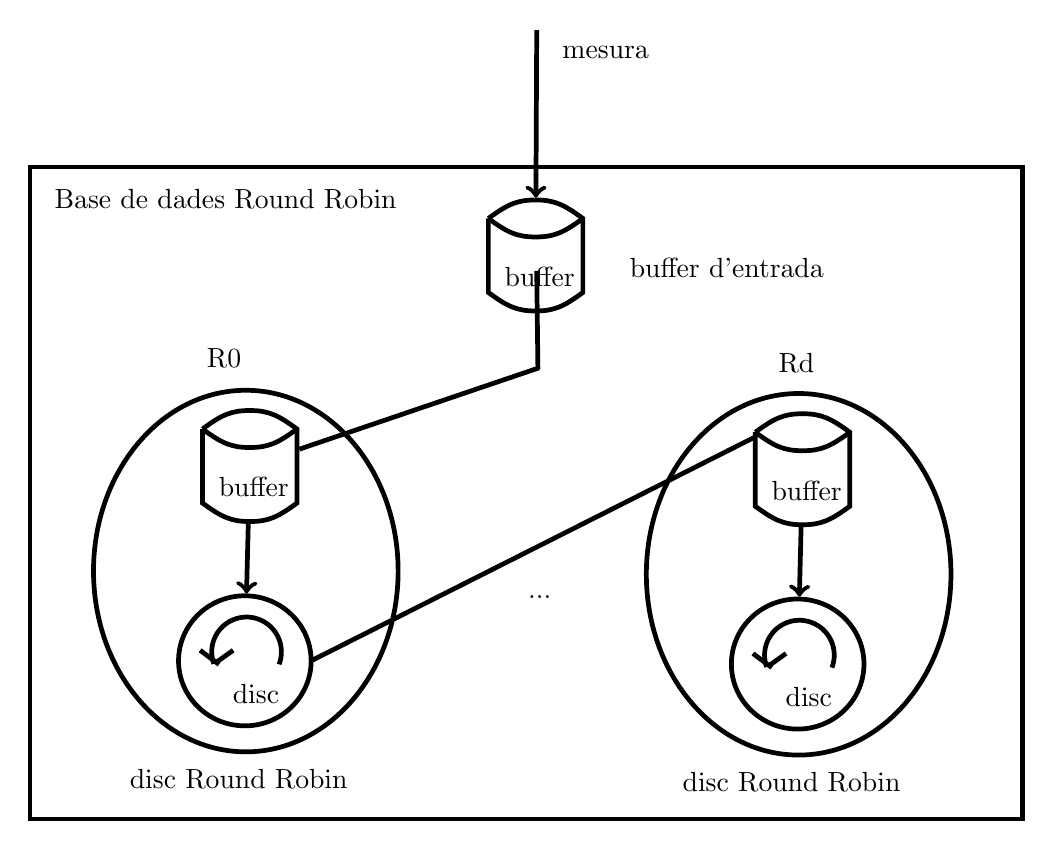
\begin{tikzpicture}
\pgftransformxscale{1.000000}
\pgftransformyscale{-1.000000}
\definecolor{dialinecolor}{rgb}{0.000000, 0.000000, 0.000000}
\pgfsetstrokecolor{dialinecolor}
\definecolor{dialinecolor}{rgb}{1.000000, 1.000000, 1.000000}
\pgfsetfillcolor{dialinecolor}
\definecolor{dialinecolor}{rgb}{1.000000, 1.000000, 1.000000}
\pgfsetfillcolor{dialinecolor}
\fill (7.200000\du,-9.403360\du)--(7.200000\du,4.396640\du)--(28.200000\du,4.396640\du)--(28.200000\du,-9.403360\du)--cycle;
\pgfsetlinewidth{0.100000\du}
\pgfsetdash{}{0pt}
\pgfsetdash{}{0pt}
\pgfsetmiterjoin
\definecolor{dialinecolor}{rgb}{0.000000, 0.000000, 0.000000}
\pgfsetstrokecolor{dialinecolor}
\draw (7.200000\du,-9.403360\du)--(7.200000\du,4.396640\du)--(28.200000\du,4.396640\du)--(28.200000\du,-9.403360\du)--cycle;
% setfont left to latex
\definecolor{dialinecolor}{rgb}{0.000000, 0.000000, 0.000000}
\pgfsetstrokecolor{dialinecolor}
\node at (17.700000\du,-2.308360\du){};
\definecolor{dialinecolor}{rgb}{1.000000, 1.000000, 1.000000}
\pgfsetfillcolor{dialinecolor}
\pgfpathellipse{\pgfpoint{11.767336\du}{-0.851678\du}}{\pgfpoint{3.224066\du}{0\du}}{\pgfpoint{0\du}{3.826682\du}}
\pgfusepath{fill}
\pgfsetlinewidth{0.100000\du}
\pgfsetdash{}{0pt}
\pgfsetdash{}{0pt}
\pgfsetmiterjoin
\definecolor{dialinecolor}{rgb}{0.000000, 0.000000, 0.000000}
\pgfsetstrokecolor{dialinecolor}
\pgfpathellipse{\pgfpoint{11.767336\du}{-0.851678\du}}{\pgfpoint{3.224066\du}{0\du}}{\pgfpoint{0\du}{3.826682\du}}
\pgfusepath{stroke}
% setfont left to latex
\definecolor{dialinecolor}{rgb}{0.000000, 0.000000, 0.000000}
\pgfsetstrokecolor{dialinecolor}
\node at (11.767336\du,-0.656678\du){};
\definecolor{dialinecolor}{rgb}{1.000000, 1.000000, 1.000000}
\pgfsetfillcolor{dialinecolor}
\pgfpathellipse{\pgfpoint{11.746664\du}{1.048318\du}}{\pgfpoint{1.403364\du}{0\du}}{\pgfpoint{0\du}{1.376682\du}}
\pgfusepath{fill}
\pgfsetlinewidth{0.100000\du}
\pgfsetdash{}{0pt}
\pgfsetdash{}{0pt}
\pgfsetmiterjoin
\definecolor{dialinecolor}{rgb}{0.000000, 0.000000, 0.000000}
\pgfsetstrokecolor{dialinecolor}
\pgfpathellipse{\pgfpoint{11.746664\du}{1.048318\du}}{\pgfpoint{1.403364\du}{0\du}}{\pgfpoint{0\du}{1.376682\du}}
\pgfusepath{stroke}
% setfont left to latex
\definecolor{dialinecolor}{rgb}{0.000000, 0.000000, 0.000000}
\pgfsetstrokecolor{dialinecolor}
\node at (11.746664\du,1.243318\du){};
\pgfsetlinewidth{0.100000\du}
\pgfsetdash{}{0pt}
\pgfsetdash{}{0pt}
\pgfsetbuttcap
\pgfsetmiterjoin
\pgfsetlinewidth{0.100000\du}
\pgfsetbuttcap
\pgfsetmiterjoin
\pgfsetdash{}{0pt}
\definecolor{dialinecolor}{rgb}{1.000000, 1.000000, 1.000000}
\pgfsetfillcolor{dialinecolor}
\pgfpathmoveto{\pgfpoint{10.850000\du}{-3.858333\du}}
\pgfpathcurveto{\pgfpoint{11.250000\du}{-4.152083\du}}{\pgfpoint{11.450000\du}{-4.250000\du}}{\pgfpoint{11.850000\du}{-4.250000\du}}
\pgfpathcurveto{\pgfpoint{12.250000\du}{-4.250000\du}}{\pgfpoint{12.450000\du}{-4.152083\du}}{\pgfpoint{12.850000\du}{-3.858333\du}}
\pgfpathlineto{\pgfpoint{12.850000\du}{-2.291667\du}}
\pgfpathcurveto{\pgfpoint{12.450000\du}{-1.997917\du}}{\pgfpoint{12.250000\du}{-1.900000\du}}{\pgfpoint{11.850000\du}{-1.900000\du}}
\pgfpathcurveto{\pgfpoint{11.450000\du}{-1.900000\du}}{\pgfpoint{11.250000\du}{-1.997917\du}}{\pgfpoint{10.850000\du}{-2.291667\du}}
\pgfpathlineto{\pgfpoint{10.850000\du}{-3.858333\du}}
\pgfusepath{fill}
\definecolor{dialinecolor}{rgb}{0.000000, 0.000000, 0.000000}
\pgfsetstrokecolor{dialinecolor}
\pgfpathmoveto{\pgfpoint{10.850000\du}{-3.858333\du}}
\pgfpathcurveto{\pgfpoint{11.250000\du}{-4.152083\du}}{\pgfpoint{11.450000\du}{-4.250000\du}}{\pgfpoint{11.850000\du}{-4.250000\du}}
\pgfpathcurveto{\pgfpoint{12.250000\du}{-4.250000\du}}{\pgfpoint{12.450000\du}{-4.152083\du}}{\pgfpoint{12.850000\du}{-3.858333\du}}
\pgfpathlineto{\pgfpoint{12.850000\du}{-2.291667\du}}
\pgfpathcurveto{\pgfpoint{12.450000\du}{-1.997917\du}}{\pgfpoint{12.250000\du}{-1.900000\du}}{\pgfpoint{11.850000\du}{-1.900000\du}}
\pgfpathcurveto{\pgfpoint{11.450000\du}{-1.900000\du}}{\pgfpoint{11.250000\du}{-1.997917\du}}{\pgfpoint{10.850000\du}{-2.291667\du}}
\pgfpathlineto{\pgfpoint{10.850000\du}{-3.858333\du}}
\pgfusepath{stroke}
\pgfsetbuttcap
\pgfsetmiterjoin
\pgfsetdash{}{0pt}
\definecolor{dialinecolor}{rgb}{0.000000, 0.000000, 0.000000}
\pgfsetstrokecolor{dialinecolor}
\pgfpathmoveto{\pgfpoint{10.850000\du}{-3.858333\du}}
\pgfpathcurveto{\pgfpoint{11.250000\du}{-3.564583\du}}{\pgfpoint{11.450000\du}{-3.466667\du}}{\pgfpoint{11.850000\du}{-3.466667\du}}
\pgfpathcurveto{\pgfpoint{12.250000\du}{-3.466667\du}}{\pgfpoint{12.450000\du}{-3.564583\du}}{\pgfpoint{12.850000\du}{-3.858333\du}}
\pgfusepath{stroke}
% setfont left to latex
\definecolor{dialinecolor}{rgb}{0.000000, 0.000000, 0.000000}
\pgfsetstrokecolor{dialinecolor}
\node at (11.850000\du,-2.679167\du){};
\pgfsetlinewidth{0.100000\du}
\pgfsetdash{}{0pt}
\pgfsetdash{}{0pt}
\pgfsetbuttcap
{
\definecolor{dialinecolor}{rgb}{0.000000, 0.000000, 0.000000}
\pgfsetfillcolor{dialinecolor}
% was here!!!
\definecolor{dialinecolor}{rgb}{0.000000, 0.000000, 0.000000}
\pgfsetstrokecolor{dialinecolor}
\pgfpathmoveto{\pgfpoint{12.471574\du}{1.123388\du}}
\pgfpatharc{21}{-200}{0.737464\du and 0.737464\du}
\pgfusepath{stroke}
}
\pgfsetlinewidth{0.100000\du}
\pgfsetdash{}{0pt}
\pgfsetdash{}{0pt}
\pgfsetbuttcap
{
\definecolor{dialinecolor}{rgb}{0.000000, 0.000000, 0.000000}
\pgfsetfillcolor{dialinecolor}
% was here!!!
\definecolor{dialinecolor}{rgb}{0.000000, 0.000000, 0.000000}
\pgfsetstrokecolor{dialinecolor}
\draw (16.171600\du,0.473318\du)--(16.171600\du,0.473318\du);
}
\pgfsetlinewidth{0.100000\du}
\pgfsetdash{}{0pt}
\pgfsetdash{}{0pt}
\pgfsetbuttcap
{
\definecolor{dialinecolor}{rgb}{0.000000, 0.000000, 0.000000}
\pgfsetfillcolor{dialinecolor}
% was here!!!
\definecolor{dialinecolor}{rgb}{0.000000, 0.000000, 0.000000}
\pgfsetstrokecolor{dialinecolor}
\draw (11.200000\du,1.125000\du)--(10.800000\du,0.825000\du);
}
\pgfsetlinewidth{0.100000\du}
\pgfsetdash{}{0pt}
\pgfsetdash{}{0pt}
\pgfsetbuttcap
{
\definecolor{dialinecolor}{rgb}{0.000000, 0.000000, 0.000000}
\pgfsetfillcolor{dialinecolor}
% was here!!!
\definecolor{dialinecolor}{rgb}{0.000000, 0.000000, 0.000000}
\pgfsetstrokecolor{dialinecolor}
\draw (11.150000\du,1.075000\du)--(11.500000\du,0.825000\du);
}
\pgfsetlinewidth{0.100000\du}
\pgfsetdash{}{0pt}
\pgfsetdash{}{0pt}
\pgfsetbuttcap
{
\definecolor{dialinecolor}{rgb}{0.000000, 0.000000, 0.000000}
\pgfsetfillcolor{dialinecolor}
% was here!!!
\pgfsetarrowsend{to}
\definecolor{dialinecolor}{rgb}{0.000000, 0.000000, 0.000000}
\pgfsetstrokecolor{dialinecolor}
\draw (11.819309\du,-1.850387\du)--(11.782400\du,-0.377629\du);
}
% setfont left to latex
\definecolor{dialinecolor}{rgb}{0.000000, 0.000000, 0.000000}
\pgfsetstrokecolor{dialinecolor}
\node[anchor=west] at (10.950000\du,-2.625000\du){buffer};
% setfont left to latex
\definecolor{dialinecolor}{rgb}{0.000000, 0.000000, 0.000000}
\pgfsetstrokecolor{dialinecolor}
\node[anchor=west] at (11.246600\du,1.748320\du){disc};
% setfont left to latex
\definecolor{dialinecolor}{rgb}{0.000000, 0.000000, 0.000000}
\pgfsetstrokecolor{dialinecolor}
\node[anchor=west] at (9.067340\du,3.548320\du){disc Round Robin};
\definecolor{dialinecolor}{rgb}{1.000000, 1.000000, 1.000000}
\pgfsetfillcolor{dialinecolor}
\pgfpathellipse{\pgfpoint{23.469066\du}{-0.783318\du}}{\pgfpoint{3.224066\du}{0\du}}{\pgfpoint{0\du}{3.826682\du}}
\pgfusepath{fill}
\pgfsetlinewidth{0.100000\du}
\pgfsetdash{}{0pt}
\pgfsetdash{}{0pt}
\pgfsetmiterjoin
\definecolor{dialinecolor}{rgb}{0.000000, 0.000000, 0.000000}
\pgfsetstrokecolor{dialinecolor}
\pgfpathellipse{\pgfpoint{23.469066\du}{-0.783318\du}}{\pgfpoint{3.224066\du}{0\du}}{\pgfpoint{0\du}{3.826682\du}}
\pgfusepath{stroke}
% setfont left to latex
\definecolor{dialinecolor}{rgb}{0.000000, 0.000000, 0.000000}
\pgfsetstrokecolor{dialinecolor}
\node at (23.469066\du,-0.588318\du){};
\definecolor{dialinecolor}{rgb}{1.000000, 1.000000, 1.000000}
\pgfsetfillcolor{dialinecolor}
\pgfpathellipse{\pgfpoint{23.448364\du}{1.116682\du}}{\pgfpoint{1.403364\du}{0\du}}{\pgfpoint{0\du}{1.376682\du}}
\pgfusepath{fill}
\pgfsetlinewidth{0.100000\du}
\pgfsetdash{}{0pt}
\pgfsetdash{}{0pt}
\pgfsetmiterjoin
\definecolor{dialinecolor}{rgb}{0.000000, 0.000000, 0.000000}
\pgfsetstrokecolor{dialinecolor}
\pgfpathellipse{\pgfpoint{23.448364\du}{1.116682\du}}{\pgfpoint{1.403364\du}{0\du}}{\pgfpoint{0\du}{1.376682\du}}
\pgfusepath{stroke}
% setfont left to latex
\definecolor{dialinecolor}{rgb}{0.000000, 0.000000, 0.000000}
\pgfsetstrokecolor{dialinecolor}
\node at (23.448364\du,1.311682\du){};
\pgfsetlinewidth{0.100000\du}
\pgfsetdash{}{0pt}
\pgfsetdash{}{0pt}
\pgfsetbuttcap
\pgfsetmiterjoin
\pgfsetlinewidth{0.100000\du}
\pgfsetbuttcap
\pgfsetmiterjoin
\pgfsetdash{}{0pt}
\definecolor{dialinecolor}{rgb}{1.000000, 1.000000, 1.000000}
\pgfsetfillcolor{dialinecolor}
\pgfpathmoveto{\pgfpoint{22.551700\du}{-3.789973\du}}
\pgfpathcurveto{\pgfpoint{22.951700\du}{-4.083723\du}}{\pgfpoint{23.151700\du}{-4.181640\du}}{\pgfpoint{23.551700\du}{-4.181640\du}}
\pgfpathcurveto{\pgfpoint{23.951700\du}{-4.181640\du}}{\pgfpoint{24.151700\du}{-4.083723\du}}{\pgfpoint{24.551700\du}{-3.789973\du}}
\pgfpathlineto{\pgfpoint{24.551700\du}{-2.223307\du}}
\pgfpathcurveto{\pgfpoint{24.151700\du}{-1.929557\du}}{\pgfpoint{23.951700\du}{-1.831640\du}}{\pgfpoint{23.551700\du}{-1.831640\du}}
\pgfpathcurveto{\pgfpoint{23.151700\du}{-1.831640\du}}{\pgfpoint{22.951700\du}{-1.929557\du}}{\pgfpoint{22.551700\du}{-2.223307\du}}
\pgfpathlineto{\pgfpoint{22.551700\du}{-3.789973\du}}
\pgfusepath{fill}
\definecolor{dialinecolor}{rgb}{0.000000, 0.000000, 0.000000}
\pgfsetstrokecolor{dialinecolor}
\pgfpathmoveto{\pgfpoint{22.551700\du}{-3.789973\du}}
\pgfpathcurveto{\pgfpoint{22.951700\du}{-4.083723\du}}{\pgfpoint{23.151700\du}{-4.181640\du}}{\pgfpoint{23.551700\du}{-4.181640\du}}
\pgfpathcurveto{\pgfpoint{23.951700\du}{-4.181640\du}}{\pgfpoint{24.151700\du}{-4.083723\du}}{\pgfpoint{24.551700\du}{-3.789973\du}}
\pgfpathlineto{\pgfpoint{24.551700\du}{-2.223307\du}}
\pgfpathcurveto{\pgfpoint{24.151700\du}{-1.929557\du}}{\pgfpoint{23.951700\du}{-1.831640\du}}{\pgfpoint{23.551700\du}{-1.831640\du}}
\pgfpathcurveto{\pgfpoint{23.151700\du}{-1.831640\du}}{\pgfpoint{22.951700\du}{-1.929557\du}}{\pgfpoint{22.551700\du}{-2.223307\du}}
\pgfpathlineto{\pgfpoint{22.551700\du}{-3.789973\du}}
\pgfusepath{stroke}
\pgfsetbuttcap
\pgfsetmiterjoin
\pgfsetdash{}{0pt}
\definecolor{dialinecolor}{rgb}{0.000000, 0.000000, 0.000000}
\pgfsetstrokecolor{dialinecolor}
\pgfpathmoveto{\pgfpoint{22.551700\du}{-3.789973\du}}
\pgfpathcurveto{\pgfpoint{22.951700\du}{-3.496223\du}}{\pgfpoint{23.151700\du}{-3.398307\du}}{\pgfpoint{23.551700\du}{-3.398307\du}}
\pgfpathcurveto{\pgfpoint{23.951700\du}{-3.398307\du}}{\pgfpoint{24.151700\du}{-3.496223\du}}{\pgfpoint{24.551700\du}{-3.789973\du}}
\pgfusepath{stroke}
% setfont left to latex
\definecolor{dialinecolor}{rgb}{0.000000, 0.000000, 0.000000}
\pgfsetstrokecolor{dialinecolor}
\node at (23.551700\du,-2.610807\du){};
\pgfsetlinewidth{0.100000\du}
\pgfsetdash{}{0pt}
\pgfsetdash{}{0pt}
\pgfsetbuttcap
{
\definecolor{dialinecolor}{rgb}{0.000000, 0.000000, 0.000000}
\pgfsetfillcolor{dialinecolor}
% was here!!!
\definecolor{dialinecolor}{rgb}{0.000000, 0.000000, 0.000000}
\pgfsetstrokecolor{dialinecolor}
\pgfpathmoveto{\pgfpoint{24.173374\du}{1.191748\du}}
\pgfpatharc{21}{-200}{0.737498\du and 0.737498\du}
\pgfusepath{stroke}
}
\pgfsetlinewidth{0.100000\du}
\pgfsetdash{}{0pt}
\pgfsetdash{}{0pt}
\pgfsetbuttcap
{
\definecolor{dialinecolor}{rgb}{0.000000, 0.000000, 0.000000}
\pgfsetfillcolor{dialinecolor}
% was here!!!
\definecolor{dialinecolor}{rgb}{0.000000, 0.000000, 0.000000}
\pgfsetstrokecolor{dialinecolor}
\draw (27.873400\du,0.541682\du)--(27.873400\du,0.541682\du);
}
\pgfsetlinewidth{0.100000\du}
\pgfsetdash{}{0pt}
\pgfsetdash{}{0pt}
\pgfsetbuttcap
{
\definecolor{dialinecolor}{rgb}{0.000000, 0.000000, 0.000000}
\pgfsetfillcolor{dialinecolor}
% was here!!!
\definecolor{dialinecolor}{rgb}{0.000000, 0.000000, 0.000000}
\pgfsetstrokecolor{dialinecolor}
\draw (22.901700\du,1.193360\du)--(22.501700\du,0.893364\du);
}
\pgfsetlinewidth{0.100000\du}
\pgfsetdash{}{0pt}
\pgfsetdash{}{0pt}
\pgfsetbuttcap
{
\definecolor{dialinecolor}{rgb}{0.000000, 0.000000, 0.000000}
\pgfsetfillcolor{dialinecolor}
% was here!!!
\definecolor{dialinecolor}{rgb}{0.000000, 0.000000, 0.000000}
\pgfsetstrokecolor{dialinecolor}
\draw (22.851700\du,1.143360\du)--(23.201700\du,0.893364\du);
}
\pgfsetlinewidth{0.100000\du}
\pgfsetdash{}{0pt}
\pgfsetdash{}{0pt}
\pgfsetbuttcap
{
\definecolor{dialinecolor}{rgb}{0.000000, 0.000000, 0.000000}
\pgfsetfillcolor{dialinecolor}
% was here!!!
\pgfsetarrowsend{to}
\definecolor{dialinecolor}{rgb}{0.000000, 0.000000, 0.000000}
\pgfsetstrokecolor{dialinecolor}
\draw (23.521009\du,-1.782025\du)--(23.484100\du,-0.309267\du);
}
% setfont left to latex
\definecolor{dialinecolor}{rgb}{0.000000, 0.000000, 0.000000}
\pgfsetstrokecolor{dialinecolor}
\node[anchor=west] at (22.651700\du,-2.556640\du){buffer};
% setfont left to latex
\definecolor{dialinecolor}{rgb}{0.000000, 0.000000, 0.000000}
\pgfsetstrokecolor{dialinecolor}
\node[anchor=west] at (22.948400\du,1.816680\du){disc};
% setfont left to latex
\definecolor{dialinecolor}{rgb}{0.000000, 0.000000, 0.000000}
\pgfsetstrokecolor{dialinecolor}
\node[anchor=west] at (20.769100\du,3.616680\du){disc Round Robin};
% setfont left to latex
\definecolor{dialinecolor}{rgb}{0.000000, 0.000000, 0.000000}
\pgfsetstrokecolor{dialinecolor}
\node[anchor=west] at (17.500000\du,-0.300000\du){...};
% setfont left to latex
\definecolor{dialinecolor}{rgb}{0.000000, 0.000000, 0.000000}
\pgfsetstrokecolor{dialinecolor}
\node[anchor=west] at (10.700000\du,-5.350000\du){R0};
% setfont left to latex
\definecolor{dialinecolor}{rgb}{0.000000, 0.000000, 0.000000}
\pgfsetstrokecolor{dialinecolor}
\node[anchor=west] at (22.800000\du,-5.250000\du){Rd};
\pgfsetlinewidth{0.100000\du}
\pgfsetdash{}{0pt}
\pgfsetdash{}{0pt}
\pgfsetbuttcap
{
\definecolor{dialinecolor}{rgb}{0.000000, 0.000000, 0.000000}
\pgfsetfillcolor{dialinecolor}
% was here!!!
\definecolor{dialinecolor}{rgb}{0.000000, 0.000000, 0.000000}
\pgfsetstrokecolor{dialinecolor}
\draw (10.123400\du,-7.233320\du)--(10.123400\du,-7.233320\du);
}
\pgfsetlinewidth{0.100000\du}
\pgfsetdash{}{0pt}
\pgfsetdash{}{0pt}
\pgfsetbuttcap
\pgfsetmiterjoin
\pgfsetlinewidth{0.100000\du}
\pgfsetbuttcap
\pgfsetmiterjoin
\pgfsetdash{}{0pt}
\definecolor{dialinecolor}{rgb}{1.000000, 1.000000, 1.000000}
\pgfsetfillcolor{dialinecolor}
\pgfpathmoveto{\pgfpoint{16.901700\du}{-8.314973\du}}
\pgfpathcurveto{\pgfpoint{17.301700\du}{-8.608723\du}}{\pgfpoint{17.501700\du}{-8.706640\du}}{\pgfpoint{17.901700\du}{-8.706640\du}}
\pgfpathcurveto{\pgfpoint{18.301700\du}{-8.706640\du}}{\pgfpoint{18.501700\du}{-8.608723\du}}{\pgfpoint{18.901700\du}{-8.314973\du}}
\pgfpathlineto{\pgfpoint{18.901700\du}{-6.748307\du}}
\pgfpathcurveto{\pgfpoint{18.501700\du}{-6.454557\du}}{\pgfpoint{18.301700\du}{-6.356640\du}}{\pgfpoint{17.901700\du}{-6.356640\du}}
\pgfpathcurveto{\pgfpoint{17.501700\du}{-6.356640\du}}{\pgfpoint{17.301700\du}{-6.454557\du}}{\pgfpoint{16.901700\du}{-6.748307\du}}
\pgfpathlineto{\pgfpoint{16.901700\du}{-8.314973\du}}
\pgfusepath{fill}
\definecolor{dialinecolor}{rgb}{0.000000, 0.000000, 0.000000}
\pgfsetstrokecolor{dialinecolor}
\pgfpathmoveto{\pgfpoint{16.901700\du}{-8.314973\du}}
\pgfpathcurveto{\pgfpoint{17.301700\du}{-8.608723\du}}{\pgfpoint{17.501700\du}{-8.706640\du}}{\pgfpoint{17.901700\du}{-8.706640\du}}
\pgfpathcurveto{\pgfpoint{18.301700\du}{-8.706640\du}}{\pgfpoint{18.501700\du}{-8.608723\du}}{\pgfpoint{18.901700\du}{-8.314973\du}}
\pgfpathlineto{\pgfpoint{18.901700\du}{-6.748307\du}}
\pgfpathcurveto{\pgfpoint{18.501700\du}{-6.454557\du}}{\pgfpoint{18.301700\du}{-6.356640\du}}{\pgfpoint{17.901700\du}{-6.356640\du}}
\pgfpathcurveto{\pgfpoint{17.501700\du}{-6.356640\du}}{\pgfpoint{17.301700\du}{-6.454557\du}}{\pgfpoint{16.901700\du}{-6.748307\du}}
\pgfpathlineto{\pgfpoint{16.901700\du}{-8.314973\du}}
\pgfusepath{stroke}
\pgfsetbuttcap
\pgfsetmiterjoin
\pgfsetdash{}{0pt}
\definecolor{dialinecolor}{rgb}{0.000000, 0.000000, 0.000000}
\pgfsetstrokecolor{dialinecolor}
\pgfpathmoveto{\pgfpoint{16.901700\du}{-8.314973\du}}
\pgfpathcurveto{\pgfpoint{17.301700\du}{-8.021223\du}}{\pgfpoint{17.501700\du}{-7.923307\du}}{\pgfpoint{17.901700\du}{-7.923307\du}}
\pgfpathcurveto{\pgfpoint{18.301700\du}{-7.923307\du}}{\pgfpoint{18.501700\du}{-8.021223\du}}{\pgfpoint{18.901700\du}{-8.314973\du}}
\pgfusepath{stroke}
% setfont left to latex
\definecolor{dialinecolor}{rgb}{0.000000, 0.000000, 0.000000}
\pgfsetstrokecolor{dialinecolor}
\node at (17.901700\du,-7.135807\du){};
% setfont left to latex
\definecolor{dialinecolor}{rgb}{0.000000, 0.000000, 0.000000}
\pgfsetstrokecolor{dialinecolor}
\node[anchor=west] at (17.001700\du,-7.081640\du){buffer};
% setfont left to latex
\definecolor{dialinecolor}{rgb}{0.000000, 0.000000, 0.000000}
\pgfsetstrokecolor{dialinecolor}
\node[anchor=west] at (19.650000\du,-7.278360\du){buffer d'entrada};
\pgfsetlinewidth{0.100000\du}
\pgfsetdash{}{0pt}
\pgfsetdash{}{0pt}
\pgfsetbuttcap
{
\definecolor{dialinecolor}{rgb}{0.000000, 0.000000, 0.000000}
\pgfsetfillcolor{dialinecolor}
% was here!!!
\definecolor{dialinecolor}{rgb}{0.000000, 0.000000, 0.000000}
\pgfsetstrokecolor{dialinecolor}
\draw (17.975000\du,-5.153360\du)--(12.900117\du,-3.431330\du);
}
\pgfsetlinewidth{0.100000\du}
\pgfsetdash{}{0pt}
\pgfsetdash{}{0pt}
\pgfsetbuttcap
{
\definecolor{dialinecolor}{rgb}{0.000000, 0.000000, 0.000000}
\pgfsetfillcolor{dialinecolor}
% was here!!!
\definecolor{dialinecolor}{rgb}{0.000000, 0.000000, 0.000000}
\pgfsetstrokecolor{dialinecolor}
\draw (17.925000\du,-7.203360\du)--(17.950000\du,-5.128360\du);
}
\pgfsetlinewidth{0.100000\du}
\pgfsetdash{}{0pt}
\pgfsetdash{}{0pt}
\pgfsetbuttcap
{
\definecolor{dialinecolor}{rgb}{0.000000, 0.000000, 0.000000}
\pgfsetfillcolor{dialinecolor}
% was here!!!
\definecolor{dialinecolor}{rgb}{0.000000, 0.000000, 0.000000}
\pgfsetstrokecolor{dialinecolor}
\draw (22.551700\du,-3.692050\du)--(13.150000\du,1.048320\du);
}
\pgfsetlinewidth{0.100000\du}
\pgfsetdash{}{0pt}
\pgfsetdash{}{0pt}
\pgfsetbuttcap
{
\definecolor{dialinecolor}{rgb}{0.000000, 0.000000, 0.000000}
\pgfsetfillcolor{dialinecolor}
% was here!!!
\pgfsetarrowsend{to}
\definecolor{dialinecolor}{rgb}{0.000000, 0.000000, 0.000000}
\pgfsetstrokecolor{dialinecolor}
\draw (17.925000\du,-12.303400\du)--(17.907673\du,-8.754869\du);
}
% setfont left to latex
\definecolor{dialinecolor}{rgb}{0.000000, 0.000000, 0.000000}
\pgfsetstrokecolor{dialinecolor}
\node[anchor=west] at (18.225000\du,-11.828400\du){mesura};
% setfont left to latex
\definecolor{dialinecolor}{rgb}{0.000000, 0.000000, 0.000000}
\pgfsetstrokecolor{dialinecolor}
\node[anchor=west] at (7.475000\du,-8.728360\du){Base de dades Round Robin};
\end{tikzpicture}

\caption{Esquema particular del model Round Robin sense emmagatzemar a buffer}
\label{fig:model:esquemanobuffer}
\end{figure}




Un concepte al qual RRDtool dedica molta importància és al de comptadors, velocitats mitjanes i magnituds, però no s'ha trobat rellevant descriure-ho com a part del model ja és fruit de l'especialitat que RRDtool té amb els comptadors. No obstant, el model RRD si que permet l'anàlisi  d'aquests sistemes, es poden configurar els paràmetres d'interpoladors i períodes de mostreig adequadament per tal que es corresponguin amb el comportament que té RRDtool.

Altres conceptes que es creu que sí que podrien formar part del model es proposen tot seguit.


\section{Treball futur}
\label{sec:futur}

El model de dades Round Robin dissenyat apropa l'àmbit de sistemes de monitoratge al de mineria de dades per sèries temporals. A partir d'aquest model, hi ha espai per investigar i desenvolupar noves tècniques que tractin les mesures que s'han adquirit en el monitoratge com a sèries temporals.


El tractament de mesures desconegudes és un bon candidat a formar part del model ja que en el monitoratge de sèries temporals no es poden evitar. Primer, s'hauria d'ampliar el conjunt de valors d'una mesura amb un valor especial que fos el 'desconegut'. Segon, de manera conjunta als buffers i als interpoladors, s'hauria de definir uns predicats que marquin quan cal considerar que el resultat d'una interpolació no pot prendre el valor calculat sinó que ha de prendre el valor 'desconegut'. Tercer, els interpoladors haurien de saber treballar interpolar quan en els intervals de consolidació hi ha mesures desconegudes. En el model RRD dissenyat es permet interpolar encara que en un interval no s'hagin pres mesures, però no es defineix com es comporta quan en un interval hi ha barrejades mesures conegudes i desconegudes.

L'operació de consulta també és un bon candidat pel model. En el model RRD s'ha definit la representació de sèries temporals exemplificada amb funcions a trossos constants. Però la representació només és la primera part de l'operació de consulta, a les bases de dades ja solen ser complicades i per sèries temporals encara més. Les consultes han de definir el comportament davant de les tasques que es recerquen en l'àmbit de les sèries temporals, com per exemple l'indexat, l'agrupament, la classificació o la segmentació,~\cite{keogh02}. Cal estudiar detingudament les tècniques que donen bons resultats i definir-les des del punt de vista del model RRD; és a dir com consultar a través dels diferents discs Round Robin, i determinar si donen bons resultats amb el model RRD.
Aquestes operacions per sèries temporals se solen basar en cercar similituds entre dues sèries temporals. Així doncs, les operacions de consulta també han de ser capaces de fusionar i calcular amb dades de dues o més bases de dades RRD.


En l'operació de consulta s'hi inclouen els procediments de predicció.  Hi ha una gran col\l.lecció de mètodes de predicció en el camp de les sèries temporals: \emph{moving average}, \emph{exponential smoothing}, \emph{Autoregressive integrated moving average} (ARIMA), etc. i s'ha de plantejar si és possible aplicar-los a una sèrie temporal que està partida amb diferents temps de mostreig, com és el cas dels diferents discs Round Robin. Els mètodes de predicció també permeten validar i reconstruir valors a la base de dades.

En el model RRD hi ha uns quants paràmetres que cal configurar per cada base de dades, com són els interpoladors, els períodes de mostreig, la quantitat de discs Round Robin, etc. En aquest sentit es pot estudiar quin efecte tenen diferents configuracions de paràmetres i plantejar la hipòtesis que donades dues bases de dades RRD per a la mateixa sèrie temporal, en una hi ha més informació. El SGBD RRDtool ha implementat el model RRD amb una configuració determinada de paràmetres de tal manera que conserva les dades segons el criteri del total; aquest s'entén molt bé per comptadors però no  per altres tipus de dades. En el model RRD, es pot estudiar amb més detall l'efecte d'aquest criteri i d'altres, com per exemple criteris que minimitzin l'error de representació.


A part del model RRD, hi ha altres tècniques que proposen solucions d'emmagatzematge per a les sèries temporals, com per exemple T-Time,~\cite{assfalg08:ttime}, o iSAX,~\cite{isax}. Es poden comparar amb el model RRD pel que fa a avantatges i inconvenients i ampliar el model RRD amb conceptes interessants que aquestes tècniques puguin tenir.

Finalment, cal comprovar quina resposta tenen els SGBD RRD amb dades utilitzades en altres experiments, com els proposats per Keogh i Kasetty,~\cite{keogh02}. Tal com recomanen, en els experiments de mineria de dades de sèries temporals s'han d'utilitzar els mateixos valors ja que sinó es pot produir una desviació interessada en les conclusions.




% LocalWords:  SGBD RRDtool Round RRD monitoratge

%%% Local Variables: 
%%% mode: latex
%%% TeX-master: "memoria"
%%% End: 
